
\documentclass[12pt, a4paper]{article}
\usepackage[margin=1in]{geometry}
\usepackage{../auxiliary/utilities/preamble}
\usepackage{booktabs}

\newcommand{\titulo}{Tarea 2: Transformadas Integrales}
\newcommand{\fecha}{11 de febrero de 2024}

\begin{document}
\sffamily
\begin{titlepage}
    \begin{center}
        
\includegraphics[width=0.15\textwidth]{../auxiliary/assets/unam.png}
        \hspace{0.6\textwidth}
        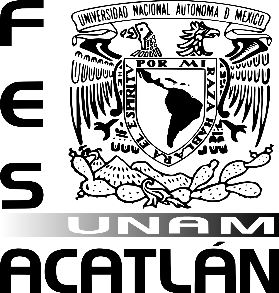
\includegraphics[width=0.15\textwidth]{../auxiliary/assets/fes.png}

        \vspace*{5cm}
        \LARGE
        \textbf{\titulo}

        \vspace{1cm}
        \large
        Camargo Badillo Luis Mauricio \\
        \vspace{1.5cm}
        \textit{\fecha}

        \vfill

        \vspace{0.5cm}
        Ecuaciones Diferenciales II \\
        Oscar Gabriel Caballero Martínez \\
        Grupo 2602 \\
        \textbf{Matemáticas Aplicadas y Computación}\\
    \end{center}
\end{titlepage}


\newpage

\section{Tabla de Transformadas Integrales}

Se solicitó la tabla disponible en \href{https://es.wikipedia.org/wiki/Transformada_integral#Tabla_de_transformadas}{el artículo de Wikipedia en español sobre las transformadas integrales}, pero con la notación utilizada en clase y reemplazando el núcleo integral por la expresión de la integral completa:

\begin{center}
    \begin{tabular}{c c c c}
        \toprule
        Nombre & Notación & Transformada & Inversa \\
        \midrule
        \\ Fourier & \(\mathcal{F}\) & \( \int_{-\infty}^{\infty} \frac{e^{-ist}}{\sqrt{2\pi}}\ f(t) dt\)  & \(\int_{-\infty}^{\infty} \frac{e^{ist}}{\sqrt{2\pi}}f(t)\ dt\) \\ \\
        \midrule
        \\ Hartley & \(\mathcal{H}\) & \(\int_{-\infty}^{\infty}\frac{\cos{(st)}+\sin{(st)}}{\sqrt{2\pi}} f(t)\ dt\) & \(\int_{-\infty}^{\infty} \frac{\cos{(st)}+\sin{(st)}}{\sqrt{2\pi}} f(t)\ dt\) \\ \\
        \midrule
        \\ Mellin & \(\mathcal{M}\) & \(\int_{0}^{\infty} t^{s-1} f(t)\ dt \) & \(\int_{c-i\infty}^{c+i\infty} \frac{t^{-s}}{2\pi i} f(t)\ dt\) \\ \\
        \midrule
        \\ Laplace Bilateral & \(\mathcal{B}\) & \(\int_{-\infty}^{\infty} e^{-st} f(t)\ dt\) & \(\int_{c-i\infty}^{c+i\infty} \frac{e^{st}}{2\pi i} f(t)\ dt\) \\ \\
        \midrule
        \\ Laplace & \(\mathcal{L}\) & \(\int_0^{\infty} e^{-st} f(t)\ dt\) & \(\int_{c-i\infty}^{c+i\infty} \frac{e^{st}}{2\pi i} f(t)\ dt\) \\ \\
        \midrule
        \\ Hankel & – & \(\int_0^{\infty} tJ_v(st) f(t)\ dt\) & \(\int_{0}^{\infty} sJ_v(st) f(t)\ dt \) \\ \\
        \midrule
        \\ Abel & – & \(\int_s^{\infty} \frac{2t}{\sqrt{t^2 - s^2}}f(t)\ dt\) & \(\int_t^{\infty} \frac{-1}{\pi\sqrt{s^2 - t^2}}\frac{d}{ds} f(t)\ dt\)\\ \\
        \midrule
        \\ Lorentz & – & \(\int_s^{\infty} \frac{2t}{\sqrt{t^2 - s^2}}f(t)\ dt\) & \(\int_t^{\infty} \frac{-1}{\pi\sqrt{s^2 - t^2}}\frac{d}{ds} f(t)\ dt\)\\ \\
        \midrule
        \\ Hilbert & \(\mathcal{H}\) & \(\int_{-\infty}^{\infty} \frac{1}{\pi}\frac{1}{s-t} f(t)\ dt\) & \(\int_{-\infty}^{\infty} \frac{1}{\pi} \frac{1}{s-t} f(t)\ dt\) \\ \\
        \bottomrule
    \end{tabular}
\end{center}

\section{Transformadas integrales de \texorpdfstring{\(f(t) = t+c\)}{f (t) = t + c}}

Además de la anterior tabla, también se solicitó la obtención de todas las transformadas integrales contenidas en ella de la función \(f(t) = t + c\).

Recordemos que en clase se demostró que toda transformada integral es lineal. Es decir, dada la forma general de una transformada integral \(T\{f(t)\}\):
\begin{align*}
    T\{t+c\} &= \int_{a}^{b} K(t,s) (t+c) \ dt \\
    &= \int_{a}^{b} K(t,s) t + K(t,s) c \ dt \\
    &= \int_{a}^{b} K(t,s) t \ dt + \int_{a}^{b} K(t,s) c \ dt \\
    &= \int_{a}^{b} K(t,s) t \ dt + c \int_{a}^{b} K(t,s) \ dt \\
    &= T\{t\} + c T\{1\}
\end{align*}
Sabiendo eso, es sumamente sencillo expresar las transformadas integrales de la función \(f(t) = t+c)\):

\begin{center}
    \begin{tabular}{c c}
        \toprule
        Nombre & Transformada t+c \\
        \midrule
        \\ Fourier \(\mathcal{F}\) & \( \int_{-\infty}^{\infty} \frac{e^{-ist}}{\sqrt{2\pi}}\ t \ dt + c \int_{-\infty}^{\infty} \frac{e^{-ist}}{\sqrt{2\pi}}\ dt\) \\ \\
        \midrule
        \\ Hartley \(\mathcal{H}\) & \(\int_{-\infty}^{\infty}\frac{\cos{(st)}+\sin{(st)}}{\sqrt{2\pi}} t \ dt + c \int_{-\infty}^{\infty}\frac{\cos{(st)}+\sin{(st)}}{\sqrt{2\pi}} \ dt\) \\ \\
        \midrule
        \\ Mellin \(\mathcal{M}\) & \(\int_{0}^{\infty} t^{s-1} t \ dt + c \int_{0}^{\infty} t^{s-1} \ dt \) \\ \\
        \midrule
        \\ Laplace Bilateral \(\mathcal{B}\) & \(\int_{-\infty}^{\infty} e^{-st} t \ dt + c \int_{-\infty}^{\infty} e^{-st} \ dt\) \\ \\
        \midrule
        \\ Laplace \(\mathcal{L}\) & \(\int_0^{\infty} e^{-st} t \ dt + c \int_0^{\infty} e^{-st} \ dt\) \\ \\
        \midrule
        \\ Hankel & \(\int_0^{\infty} tJ_v(st) t \ dt + c \int_0^{\infty} tJ_v(st) \ dt\) \\ \\
        \midrule
        \\ Abel & \(\int_s^{\infty} \frac{2t}{\sqrt{t^2 - s^2}} t \ dt + c \int_s^{\infty} \frac{2t}{\sqrt{t^2 - s^2}} \ dt\) \\ \\
        \midrule
        \\ Lorentz & \(\int_s^{\infty} \frac{2t}{\sqrt{t^2 - s^2}} t \ dt + c \int_s^{\infty} \frac{2t}{\sqrt{t^2 - s^2}} \ dt\) \\ \\
        \midrule
        \\ Hilbert \(\mathcal{H}\) & \(\int_{-\infty}^{\infty} \frac{1}{\pi}\frac{1}{s-t} t \ dt + c \int_{-\infty}^{\infty} \frac{1}{\pi}\frac{1}{s-t} \ dt\) \\ \\
        \bottomrule
    \end{tabular}
\end{center}

\end{document}
